%                      Code_Saturne version 1.3
%                      ------------------------
%
%     This file is part of the Code_Saturne Kernel, element of the
%     Code_Saturne CFD tool.
%
%     Copyright (C) 1998-2007 EDF S.A., France
%
%     contact: saturne-support@edf.fr
%
%     The Code_Saturne Kernel is free software; you can redistribute it
%     and/or modify it under the terms of the GNU General Public License
%     as published by the Free Software Foundation; either version 2 of
%     the License, or (at your option) any later version.
%
%     The Code_Saturne Kernel is distributed in the hope that it will be
%     useful, but WITHOUT ANY WARRANTY; without even the implied warranty
%     of MERCHANTABILITY or FITNESS FOR A PARTICULAR PURPOSE.  See the
%     GNU General Public License for more details.
%
%     You should have received a copy of the GNU General Public License
%     along with the Code_Saturne Kernel; if not, write to the
%     Free Software Foundation, Inc.,
%     51 Franklin St, Fifth Floor,
%     Boston, MA  02110-1301  USA
%
%-----------------------------------------------------------------------
%
\begin{center}
\underline{{\Huge \textbf{Introduction}}}
\end{center}

\vspace{1cm}

%%%%%%%%%%%%%%%%%%%%%%%%%%%%%%%%%%
%%%%%%%%%%%%%%%%%%%%%%%%%%%%%%%%%%
\section{Disclaimer}
%%%%%%%%%%%%%%%%%%%%%%%%%%%%%%%%%%
%%%%%%%%%%%%%%%%%%%%%%%%%%%%%%%%%%
\CS\ is free software; you can redistribute it
and/or modify it under the terms of the GNU General Public License
as published by the Free Software Foundation; either version 2 of
the License, or (at your option) any later version.

\CS\ is distributed in the hope that it will be
useful, but WITHOUT ANY WARRANTY; without even the implied warranty
of MERCHANTABILITY or FITNESS FOR A PARTICULAR PURPOSE.  See the
GNU General Public License for more details.\footnote{You should have
received a copy of the GNU General Public License
along with \CS; if not, write to the
Free Software Foundation, Inc.,
51 Franklin St, Fifth Floor,
Boston, MA  02110-1301  USA}

%%%%%%%%%%%%%%%%%%%%%%%%%%%%%%%%%%
%%%%%%%%%%%%%%%%%%%%%%%%%%%%%%%%%%
\section{Aims of the document}
%%%%%%%%%%%%%%%%%%%%%%%%%%%%%%%%%%
%%%%%%%%%%%%%%%%%%%%%%%%%%%%%%%%%%

This chapter constitutes an introduction to the theory and developer's guide
associated with the kernel of \CS.
The system of equations considered consists of the
Navier-Stokes equations, with turbulence and passive scalars. First, the
continuous equations for mass, momentum, turbulence and passive scalars are
presented. Then, information related to the time scheme is supplied.
Finally, the spatial discretisation is detailed: it is based on a co-located%
\footnote{%
All the variables are located at the centres of the cells.} finite volume
scheme for unstructured meshes.

To make the documentation immediately suitable to the developers' needs, it
has been organized into sub-sections corresponding to the major steps of the
algorithm and to some important subroutines of the code.

In each sub-section (for each subroutine), the \textbf{function} of the
piece of code considered is indicated. Then, a description of the \textbf{%
discretisation} follows. Finally, and more oriented towards the developers,
details of the \textbf{implementation} are provided and a list of open
problems is given (improvements, limitations...).

Several accessibility levels have been defined for the documentation, so
that it is possible to choose the information level best suited to the
intended use. At the present time, on UNIX and Linux platforms, free access
is granted to all information (level called ''\texttt{Complet}''). The most
restrictive level provides only the function of the subroutines (''\texttt{%
Fonction}'' level). The intermediate level provides the function of the
subroutines and the associated discretisation (''\texttt{Discret}'' level).

% fa modification (no more 1.1.0.m, no more "only basic")
%The current version of this documentation details the basic algorithms
%of the code and it was therefore important to be well explained by an EDF report.
During the development process of the code, the documentation is naturally
updated as and when required by the evolution of the source code itself.
Suggestions for improvement are welcome. In particular, it will be necessary
to deal with some transverse subjects (such as parallelism, periodicity or
memory management) which were voluntarily left out of the first versions, to
focus on the algorithms and their implementation.

To make it easier for the developers to keep the documentation up to date
during the development process, the files have been associated "physically"
with the release of the code (each release of the code includes a directory
containing the whole documentation). In practice,
% fa modification : discard (from the development version 1.1.0.n on),
the users of \CS\ will find the documentation at the following location
% fa modification (MFTT-MFEE)
(UNIX and Linux server at MFEE): % fa modification (SC -> CS)

\begin{center}
\texttt{\$CS\_HOME/doc/NOYAU/Postscripts/Base},
\end{center}

The general command \texttt{info\_cs [noyau]} also provides this
information.

\newpage %%%%%%%%%%%%%%%%%%%%%%%%%%%%%%%%%%
%%%%%%%%%%%%%%%%%%%%%%%%%%%%%%%%%%

\section{Continuous equations}

%%%%%%%%%%%%%%%%%%%%%%%%%%%%%%%%%%
%%%%%%%%%%%%%%%%%%%%%%%%%%%%%%%%%%

This section presents the continuous equations. It is no substitutes for the
specific sub-sections of this documentation: the purpose here is mainly to
provide an overview before more detailed reading.

In the following, $\rho $ stands for the density, $\vect{u}$ for the
velocity field. A mass source term, $\Gamma $ , may present, but in most
cases the right-hand side of the Masss equation is $\Gamma =0$

%\clearpage
\textbf{Mass}\newline
\begin{equation}
\dive(\rho \vect{u})=\Gamma
\end{equation}

In fact, to compute a given unknown $\phi$ (and in particular for the
velocity prediction), the equation $\displaystyle \frac{\partial \rho}{%
\partial t} + \dive(\rho \vect{u}) = \Gamma$ is used to re-write the term $%
\displaystyle \frac{\partial \rho\,\phi}{\partial t}$ as follows:
\mbox{$\displaystyle \rho\frac{\partial  \phi}{\partial t} - \phi\,\dive(\rho \vect{u})
+ \Gamma\,\phi$}. The possible variations in time of the density are however
not taken into account in the pressure correction step.

\clearpage \textbf{Momentum}
\begin{equation}
\left\{
\begin{array}{l}
\displaystyle\frac{\partial }{\partial t}(\rho \vect{u})+\dive(\rho \,%
\vect{u}\otimes \vect{u})=\dive(\tens{\sigma})+\vect{ST}-\tens{K}\,\vect{u}
\\
\dive(\rho \vect{u})=0%
\end{array}%
\right.
\end{equation}

$[\,\vect{ST}-\tens{K}\,\vect{u}\,]$ stands for the additional momentum
Source Terms which may be prescribed by the user (head loss, $\Gamma \vect{u}%
^{i}$ contribution associated with a user-prescribed mass source term...).

$\tens{K}$ is a positive diagonal tensor, by definition (derived, for
example, from the diagonal source term of the head loss tensor).

$\bullet $ For laminar flow, $\tens{\sigma}$ is the stress tensor:
\begin{equation}
\tens{\sigma}=\tens{\tau}-P\tens{Id}
\end{equation}%
where $\tens{\tau}$ is the viscous stress tensor, defined from $\mu =\mu
_{l} $ (dynamic molecular viscosity) and $\tens{S}$ (strain rate tensor) as:
\begin{equation}
\tens{\tau}=2\,\mu \ \tens{S}-\frac{2}{3}\mu \ tr(\tens{S})\ \tens{Id}\text{
\hspace*{1cm}with \hspace*{1cm} }\tens{S}=\frac{1}{2}(\ggrad\vect{u}+\,^{t}%
\ggrad\vect{u})  \label{Base_Introd_tau_eq}
\end{equation}

$\bullet$ For turbulent flow, $\displaystyle \tens{\sigma}$ also accounts
for the turbulent Reynolds stress tensor (correlations of the velocity
fluctuations arising from the non linear convective term). The modelling of
the latter depends upon the turbulence model adopted:

\hspace*{1cm} - with an eddy-viscosity model (EVM) such as the $%
k-\varepsilon $ model, the closure requires a turbulent viscosity $\mu _{t}$%
. With formally the same definition for $\tens{\tau}$ as in equation~(\ref%
{tau_eq}), but with $\mu =\mu _{l}+\mu _{t}$, $\tens{\sigma}$ reads:
\begin{equation}
\tens{\sigma}=\tens{\tau}-(P+\frac{2}{3}\rho k)\tens{Id}
\end{equation}

\hspace*{1cm} - with the $LES$ approach, the definition for $\tens{\sigma}$
remains the same as for the EVM, above, but the turbulent viscosity $\mu
_{t} $ now accounts only for the sub-grid effects.

\hspace*{1cm} - with a Differential Reynolds Stress Model (DRSM), the
components of the Reynolds stress tensor $\tens{R}$ are solved as extra
variables during the simulation, and are readily available for the momentum
equation, so one obtains, with $\mu =\mu _{l}$ in the definition of $%
\tens{\tau}$ (equation~(\ref{Base_Introd_tau_eq}))~:
\begin{equation}
\tens{\sigma}=\tens{\tau}-P\tens{Id}-\rho \tens{R}
\end{equation}

\hspace*{1cm}

In the following, only three standard types of turbulence models are
described, as representatives of the types of equations that need to be
dicretised. A more detailed description of available turbulence models is
described in section (?? Turbulence Models??)

\clearpage \textbf{Equations for the variables $k$ and $\varepsilon$
(standard $k-\varepsilon$ model)}

\begin{equation}
\left\{
\begin{array}{l}
\displaystyle\frac{\partial }{\partial t}(\rho k)+\dive\left[ \rho \vect{u}%
\,k-(\mu +\frac{\mu _{t}}{\sigma _{k}}\grad{k})\right] =\mathcal{P}+\mathcal{%
G}-\rho \varepsilon +\Gamma k^{i}+ST_{k} \\
\displaystyle\frac{\partial }{\partial t}(\rho \varepsilon )+\dive\left[
\rho \vect{u}\,\varepsilon -(\mu +\frac{\mu _{t}}{\sigma _{\varepsilon }}%
\grad{\varepsilon})\right] =C_{\varepsilon _{1}}\frac{\varepsilon }{k}\left[
\mathcal{P}+(1-C_{\varepsilon _{3}})\mathcal{G}\right] -\rho C_{\varepsilon
_{2}}\frac{\varepsilon ^{2}}{k}+\Gamma \varepsilon ^{i}+TS_{\varepsilon }%
\end{array}%
\right.
\end{equation}

$\mathcal{P}$ is the production term created by mean shear:
\[
\begin{array}{rcl}
\mathcal{P} & = & \displaystyle -\rho R_{ij}\frac{\partial u_i}{\partial x_j}
= -\left[-\mu_t \left(\frac{\partial u_i}{\partial x_j} + \frac{\partial u_j%
}{\partial x_i}\right) +\frac{2}{3}\mu_t\frac{\partial u_k}{\partial x_k}%
\delta_{ij} +\frac{2}{3}\rho k\delta_{ij}\right] \frac{\partial u_i}{%
\partial x_j} \\
& = & \displaystyle \mu_t \left(\frac{\partial u_i}{\partial x_j} + \frac{%
\partial u_j}{\partial x_i}\right)\frac{\partial u_i}{\partial x_j} -\frac{2%
}{3}\mu_t(\dive\vect{u})^2-\frac{2}{3}\rho k \dive(\vect{u}) \\
& = & \displaystyle \mu_t \left[ 2\left(\frac{\partial u}{\partial x}%
\right)^2+ 2\left(\frac{\partial v}{\partial y}\right)^2+ 2\left(\frac{%
\partial w}{\partial z}\right)^2+ \left(\frac{\partial u}{\partial y}+\frac{%
\partial v}{\partial x}\right)^2+ \left(\frac{\partial u}{\partial z}+\frac{%
\partial w}{\partial x}\right)^2+ \left(\frac{\partial v}{\partial z}+\frac{%
\partial w}{\partial y}\right)^2 \right] \\
\multicolumn{3}{r}{\displaystyle -\frac{2}{3}\mu_t(\dive\vect{u})^2-\frac{2}{%
3}\rho k \dive(\vect{u})}%
\end{array}
\]

$\mathcal{G}$ is the production term created by gravity effects: $%
\displaystyle \mathcal{G}=-\frac{1}{\rho}\frac{\mu_t}{\sigma_t} \frac{%
\partial\rho}{\partial x_i}g_i$

The turbulent viscosity is: $\displaystyle \mu_t=\rho C_\mu\frac{k^2}{%
\varepsilon}$.

$ST_{\varphi }$ ($\varphi =k$ or $\varepsilon $) stands for the additional
source terms prescribed by the user (in rare cases only).

The constants of the model are given below:\newline
\begin{table}[htp]
\begin{center}
\begin{tabular}{|p{0,8cm}|p{0,8cm}|p{0,8cm}|p{0,8cm}|p{0,8cm}|}
\hline
$C_\mu$ & $C_{\varepsilon_1}$ & $C_{\varepsilon_2}$ & $\sigma_k$ & $%
\sigma_\varepsilon$ \\ \hline
$0,09$ & $1,44$ & $1,92$ & $1$ & $1,3$ \\ \hline
\end{tabular}%
\end{center}
\end{table}

$C_{\varepsilon_3}=0$ if $\mathcal{G}\geqslant0$ (unstable stratification)
and $C_{\varepsilon_3}=1$ if $\mathcal{G}\leqslant0$ (stable stratification).

\clearpage \textbf{Equations for the Reynolds stress tensor components $%
R_{ij}$ and $\varepsilon$ (LRR model)}

\begin{equation}
\left\{
\begin{array}{lll}
\displaystyle\frac{\partial }{\partial t}(\rho R_{ij})+\dive(\rho \vect{u}%
\,R_{ij}-\mu \grad{R_{ij}}) & =\mathcal{P}_{ij}+G_{ij}+\Phi _{ij}+\mathit{{d}%
_{ij}-\rho \varepsilon _{ij}} & \displaystyle+\Gamma R_{ij}^{i}+ST_{R_{ij}}
\\
\displaystyle\frac{\partial }{\partial t}(\rho \varepsilon )+\dive\left[
\rho \vect{u}\,\varepsilon -(\mu \grad{\varepsilon})\right]  & =\displaystyle%
\mathit{{d}+C_{\varepsilon _{1}}\frac{\varepsilon }{k}\left[ \mathcal{P}%
+G_{\varepsilon }\right] -\rho C_{\varepsilon _{2}}\frac{\varepsilon ^{2}}{k}%
} & \displaystyle+\Gamma \varepsilon ^{i}+ST_{\varepsilon }%
\end{array}%
\right.
\end{equation}

$\tens{\mathcal{P}}$ stands for the turbulence production tensor associated
with mean flow strain-rate and $\tens{\mathcal{G}}$ is stands for the
production- tensor associated with buoyancy effects:
\begin{equation}
\displaystyle P_{ij}=\displaystyle-\rho \left[ R_{ik}\frac{\partial u_{j}}{%
\partial x_{k}}+R_{jk}\frac{\partial u_{i}}{\partial x_{k}}\right] \text{%
\hspace*{1cm}and\hspace*{1cm}}G_{ij}=-\frac{3}{2}\frac{C_{\mu }}{\sigma _{t}}%
\frac{k}{\varepsilon }(r_{i}g_{j}+r_{j}g_{i})
\end{equation}

\begin{eqnarray}
\text{with\hspace*{0cm}}\displaystyle k &=&\frac{1}{2}R_{ll}\text{%
\hspace*{0cm}and\hspace*{0cm}}\displaystyle r_{i}=R_{ik}\frac{\partial \rho
}{\partial x_{k}} \\
\text{moreover,  }\mathcal{P} &=&\frac{1}{2}\mathcal{P}_{kk}\text{%
\hspace*{1cm}and\hspace*{1cm}}G_{\varepsilon }=max(0,\frac{1}{2}G_{kk})
\end{eqnarray}

$\tens{\Phi}$ is the term representing pressure-velocity correlations:
\begin{equation}
\displaystyle\Phi _{ij}=\phi _{ij,1}+\phi _{ij,2}+\phi _{ij,3}+\phi _{ij,w}
\end{equation}%
\begin{equation}
\text{with\hspace*{0cm}}\phi _{ij,1}=-\rho \,C_{1}\frac{\varepsilon }{k}%
(R_{ij}-\frac{2}{3}k\delta _{ij})\text{\ \ , \ }\phi _{ij,2}=-\rho \,C_{2}(%
\mathcal{P}_{ij}-\frac{2}{3}\mathcal{P})\delta _{ij}\text{\ \ \ and\ \ }\phi
_{ij,3}=-C_{3}(G_{ij}-\frac{1}{3}\delta _{ij}G_{kk})
\end{equation}

The term $\phi _{ij,w}$ is called ``wall echo term'' (by default, it is not
accounted for~: see \fort{turrij}).

The dissipation term, $\varepsilon _{ij}$ , is considered isotropic:

\begin{equation}
\displaystyle\varepsilon _{ij}=\frac{2}{3}\ \delta _{ij}\varepsilon
\end{equation}

The turbulent diffusion terms are~:
\begin{equation}
d_{ij}=C_{S}\frac{\partial }{\partial x_{k}}(\rho \frac{k}{\varepsilon }%
R_{km}\frac{\partial R_{ij}}{\partial x_{m}})\text{\hspace*{1cm}and%
\hspace*{1cm}}{d}=C_{\varepsilon }\displaystyle\frac{\partial }{\partial
x_{k}}\left( \rho \frac{k}{\varepsilon }R_{km}\frac{\partial \varepsilon }{%
\partial x_{m}}\right)
\end{equation}

In the rare event of masse sources, $\Gamma R_{ij}^{i}$ and $\Gamma
\varepsilon ^{i}$ are the corresponding injection terms. $ST_{R_{ij}}$ and $%
ST_{\varepsilon }$ are also rarely used additional source terms that can
prescribed by the user.

%\begin{table}[htp]

\begin{center}
\begin{tabular}{|p{0,8cm}|p{0,8cm}|p{0,8cm}|p{0,8cm}|p{0,8cm}|p{0,8cm}|p{0,8cm}|p{0,8cm}|p{0,8cm}|p{0,8cm}|}
\hline
$C_\mu$ & $C_{\varepsilon}$ & $C_{\varepsilon_1}$ & $C_{\varepsilon_2}$ & $%
C_1$ & $C_2$ & $C_3$ & $C_S$ & $C^{\prime}_1$ & $C^{\prime}_2$ \\ \hline
$0,09$ & $0,18$ & $1,44$ & $1,92$ & $1,8$ & $0,6$ & $0,55$ & $0.22$ & $0,5$
& $0,3$ \\ \hline
\end{tabular}
\end{center}

%\end{table}

\clearpage \textbf{Definition of $\mu_t$ for $LES$}

{\tiny $\bigstar $} \underline{Smagorinsky model}
\begin{equation}
\mu _{t}=\rho \,(C_{s}\,\overline{\Delta })^{2}\sqrt{2\overline{S_{ij}}\,%
\overline{S_{ij}}}
\end{equation}%
With $\overline{S_{ij}}$ the filtered strain rate tensor components:
\begin{equation}
\overline{S_{ij}}=\frac{1}{2}\left( \frac{\partial \,\overline{u_{i}}}{%
\partial \,x_{j}}+\frac{\partial \,\overline{u_{j}}}{\partial \,x_{i}}%
\right)
\end{equation}%
Here, $\overline{u_{i}}$ stands for the $i^{th}$ resolved velocity component%
\footnote{%
In the case of implicit filtering, the discretisation in space introduces a
spectral low pass filter: only the structures larger that twice the size of
the cells are accounted for. Those structures are called ''the resolved
scales'', whereas the rest, $u_{i}-\overline{u_{i}}$, is referred to as
''unresolved scales'' or ''sub-grid scales''. The influence of the
unresolved scales on the resolved scales have to be modelled.}. \newline
\newline
$C$ is the Smagorinsky constant. Its theoretical value is $0.18$ for
homogenous isotropic turbulence, but the value $0.065$ is classic for
channel flow. \newline
\newline
$\overline{\Delta }$ is the filter width associated with the finite volume
formulation (implicit filtering which corresponds to the integration over a
cell). The value recommended for hexahedral cells is: $\overline{\Delta }%
=2\,|\Omega |^{\frac{1}{3}}$where $|\Omega |$ is the volume of the cell.

{\tiny $\bigstar $} \underline{Classic dynamic model} \ \ \ (??this should
be moved to chapter turbulence models??) \newline
\newline
A second filter is introduced: it is an explicit filter with a
characteristic width $\widetilde{\Delta }$ superior to that of the implicit
filter ($\overline{\Delta }$). If $a$ is a discrete variable defined over
the computational domain, the variable obtained after applying the explicit
filter to $a$ is noted $\tilde{a}$. Moreover, with:
\[
L_{ij}=\widetilde{\overline{u_{i}}\ \overline{u_{j}}}-\widetilde{\overline{%
u_{i}}}\ \widetilde{\overline{u_{j}}}
\]%
\[
\tau _{ij}=\overline{u_{i}u_{j}}-\overline{u_{i}}\ \overline{u_{j}}
\]%
\[
T_{ij}=\widetilde{\overline{u_{i}u_{j}}}-\widetilde{\overline{u_{i}}}\
\widetilde{\overline{u_{j}}}
\]%
Germano identity reads:
\[
L_{ij}=T_{ij}-\widetilde{\tau _{ij}}
\]

Both dynamic models described herafter rely on the estimation of the tensors
$\tens{T}$ and $\tens{\tau}$ as functions of the filter widths and of the
strain rate tensor (Smagorinsky model). The following modelling is adopted%
\footnote{$\delta_{ij}$ stands for the Kroeneker symbol.}:

\[
T_{ij}-\frac{1}{3}\delta_{ij} T_{kk}= -2 C \widetilde{\Delta}^2 |\widetilde{%
\overline{D_{ij}}}| \widetilde{\overline{D_{ij}}}
\]
\[
\tau_{ij}-\frac{1}{3}\delta_{ij} \tau_{kk}= -2 C^* \overline{\Delta}^2 |%
\overline{D_{ij}}| \overline{D_{ij}}
\]

$\overline{u}$ stands for the "implicit-filtered" value of a variable $u$
defined at the centres of the cells and $\overline{u}$ represents the
"explicit-filtered" value associated with the variable $u$. It follows that
the numerical computation of $L_{ij}$ is possible, since it requires the
explicit filtering to be applied to implicitly filtered variables only (%
\textit{i.e.} to the variables explicitly computed).

On the following assumption:

\[
C = C^*
\]

and assuming that $C^*$ is only slightly non-uniform, so that it can be
taken out of the explicit filtering operator, the following equation is
obtained:

\[
L_{ij} -\frac{1}{3} \delta_{ij} L_{kk}= C (\alpha_{ij}-\widetilde{\beta}%
_{ij})
\]

with:

\[
\alpha_{ij} = -2 \widetilde{\Delta}^2 |\widetilde{\overline{D_{ij}}}|
\widetilde{\overline{D_{ij}}}
\]
\[
\beta_{ij} = -2 \overline{\Delta}^2 |\overline{D_{ij}}| \overline{D_{ij}}
\]

Since we are left with six equations to determine one single variable, the
least square method is used\footnote{$L_{kk}$ has no effect for
incompressible flows.}. With:
\[
E_{ij} = L_{ij}-C(\alpha_{ij} - \widetilde{\beta}_{ij})
\]
the value for $C$ is obtained by solving the following equation:
\[
\frac {\partial E_{ij}E_{ij}}{\partial C} = 0
\]

Finally:
\[
C = \frac{M_{ij}L_{ij}} {M_{kl}M_{kl}}
\]
with
\[
M_{ij} = \alpha_{ij} - \widetilde{\beta}_{ij}
\]

This method allows to calculate the Smagorinsky "constant" dynamically at
each time step and at each cell. However, the value obtained for $C$ can be
subjected to strong variations. Hence, this approach is often restricted to
flows presenting one or more homogeneous directions (Homogeneous Isotropic
Turbulence, 2D flows presenting an homogeneous spanwise direction...):
indeed, in such cases, the model can be (and is) stabilized by replacing $C$
by an average value of $C$ computed over the homogeneous direction(s).

For a general case (without any homogeneous direction), a specific averaging
is introduced to stabilize the model: for any given cell of the mesh, the
averaged Smagorinsky constant is obtained as an average of $C$ over the
"extended neighbourhood" of the cell (the set of cells that share at least
one vertex with the cell considered). More precisely, the average value
(also denoted $C$ hereafter) is calculated as indicated below:

\[
C = \frac{\widetilde{M_{ij}L_{ij}}} {\widetilde{M_{kl}M_{kl}}}
\]

\clearpage \textbf{Equations for the scalars}

Two types of transport equations are considered: \newline
{\tiny $\bigstar $} advection of a scalar with additional source terms:
\begin{equation}
\frac{\partial (\rho a)}{\partial t}+\underbrace{\,\dive\,((\rho \underline{u%
})\,a)}_{\text{convection}}-\underbrace{\,\dive\,(K\grad a)}_{\text{diffusion%
}}=TS_{a}+\Gamma \,a^{i}
\end{equation}%
{\tiny $\bigstar $} advection of the variance $\widetilde{{a"}^{2}}$ with
additional source terms ~:
\begin{equation}
\begin{array}{lcl}
& \displaystyle\frac{\partial (\rho \widetilde{{a"}^{2}})}{\partial t}+%
\underbrace{\dive\,((\rho \,\underline{u})\ \widetilde{{a"}^{2}})}_{\text{%
convection}}-\underbrace{\dive\,(K\ \grad\widetilde{{a"}^{2}})}_{\text{%
diffusion}}=TS_{\widetilde{{a"}^{2}}}+\ \Gamma \,\widetilde{{a"}^{2}}^{i} &
\\
& \displaystyle\underbrace{+2\,\frac{\mu _{t}}{\sigma _{t}}(\grad\widetilde{a%
})^{2}-\frac{\rho \,\varepsilon }{R_{f}k}\ \widetilde{{a"}^{2}}}_{\text{%
production and dissipation}} &
\end{array}%
\end{equation}%
The two previous equations can be unified formally as:
\begin{equation}
\frac{\partial (\rho f)}{\partial t}+\dive\,((\rho \,\underline{u})f)-\dive%
\,(K\grad f)=TS_{f}+\Gamma \,f^{i}+T_{s}^{\,pd}  \label{Base_Introd_depart}
\end{equation}%
with:
\begin{equation}
\begin{array}{lll}
& \displaystyle T_{s}^{\,pd}=\begin{cases} 0 & \text{for $f=a$}, \\ 2\
\displaystyle \frac{\mu_t}{\sigma_t}(\grad \widetilde{a})^2 - \displaystyle
\frac{\rho\,\varepsilon}{R_f k}\ \widetilde{{a"}^2} & \text{for
$f=\widetilde{{a"}^2}$ } \end{cases} &
\end{array}%
\end{equation}

$TS_f$ represents the additional source terms that may be prescribed by the
user.

\newpage %%%%%%%%%%%%%%%%%%%%%%%%%%%%%%%%%%
%%%%%%%%%%%%%%%%%%%%%%%%%%%%%%%%%%

\section{Discretisation in time}

%%%%%%%%%%%%%%%%%%%%%%%%%%%%%%%%%%
%%%%%%%%%%%%%%%%%%%%%%%%%%%%%%%%%%
At first, the physical properties of the flow are computed (density,
viscosity, specific heat...): indeed, they may depend upon the variables
(such as the temperature for example).

The time scheme is a $\theta$-scheme:
\begin{equation}
\left\{%
\begin{array}{ll}
\theta = 1 & \text{for an implicit first order Euler scheme} \\
\theta = 1/2 & \text{for second order Crank-Nicolson scheme}%
\end{array}
\right.
\end{equation}

For the second order scheme, the time step is assumed to be constant.

A fractional step scheme is used to solve the mass and momentum equations
(Chorin). The first step (predictor step) provides predicted velocity
components: they are determined sequentially and without coupling between
each other. The mass equation is taken into account during the second step
(corrector step): a pressure Poisson equation is solved and the mass fluxes
at the cell faces are updated.

If required, the equations for the turbulent variables are solved (turbulent
kinetic energy and dissipation or Reynolds stresses and dissipation), using
a $\theta$-scheme again. For the $k-\varepsilon$ model, an additional step
is carried out to couple the source terms. For the Reynolds stress model,
the variables (turbulent stresses and dissipation) are solved sequentially,
without coupling.

Next, the equations for the ``scalars'' (enthalpy, temperature, tracers,
concentrations, mass fractions...) are solved, also with a $\theta$-scheme.

Finally, all the variables are updated and another time step may start.

The general equation for advection (valid for the velocity components, the
turbulent variables and the scalars) is re-written as follows in a condensed
form; the mass equation ($\frac{\partial \rho } {\partial t}+ \dive(\rho
\underline{u}) = \Gamma$) has been used to split the time derivative:
\begin{equation}  \label{Base_Introd_simple}
\rho \frac {\partial f}{\partial t} + \dive\,((\rho\,\underline{u}) f) - %
\dive\,(K \grad f) = S_{i}(\Phi,\varphi)\,f + S_{e}(\Phi,\varphi) + \dive%
\,(\rho\,\underline{u})\,f
\end{equation}
In this equation:\newline
\begin{tabular}{ll}
$\Phi$ & : represents the physical properties $(\rho,K,\mu_{t},...)$ \\
$\varphi$ & : represents the variables of the problem $(\vect{u}%
,k,\epsilon,...)$ \\
$S_{i}(\Phi,\varphi)\,f$ & : represents the linear part of the source terms
\\
$S_{e}(\Phi,\varphi)$ & : includes all other source terms \\
$\dive\,(\rho\,\underline{u})\,f$ & : is the term associated with ``mass
accumulation''%
\end{tabular}
\newline
\newline

The time at which the different quantities are evaluated is indicated below:%
\newline
$\bullet$ $\Phi$: the time considered is defined by the time scheme applied
to the physical properties.\newline
$\bullet$ $(\rho\,\underline{u})$: the time considered is defined by the
time scheme applied to the mass flux.\newline
$\bullet$ $S_{e}(\Phi,\varphi)$: the time considered is defined by the time
scheme applied to the explicit source terms.

If $\theta=1/2$, or if an extrapolation is used, the time step $\Delta t$ is
constant in time and uniform in space.

\subsection{Physical properties}

The physical properties of the flow (density, viscosity, specific heat...)
are:

\begin{itemize}
\item[-] either explicit, defined at the time step $n$.

\item[-] or extrapolated at $n+\theta _{\Phi }$ using the Adam-Bashforth
time scheme (in this case, the time step is assumed to be constant).
\end{itemize}

Under a more general form, this reads:
\begin{equation}
\Phi \equiv \Phi^{n+\theta_{\Phi}}=(1+\theta_{\Phi})\,\Phi^{n}-
\theta_{\Phi}\,\Phi^{n-1}
\end{equation}

\begin{equation}
\left\{%
\begin{array}{ll}
\theta_{\Phi} = 0 & \text{standard explicit formulation} \\
\theta_{\Phi} = 1/2 & \text{second order extrapolation at } n+1/2 \\
\theta_{\Phi} = 1 & \text{first order extrapolation at } n+1%
\end{array}
\right.
\end{equation}

\subsection{Mass flux}

For the mass flux, three time schemes are available. The mass flux may be:

\begin{itemize}
\item[-] explicit, taken at time step $n$ for the momentum equations and
updated with its value at time step $n+1$ for the equations for turbulence
and scalars (standard scheme).\newline

\item[-] explicit, taken at time step $n$ for the momentum equations and
also for the equations for turbulence and scalars.

\item[-] taken at $n+\theta_{F}$ (second order if $\theta_{F}=1/2$). To
solve the momentum equations, $(\rho\,\underline{u})^{n-2+\theta_{F}}$ and $%
(\rho\,\underline{u})^{n-1+\theta_{F}}$ are known. Hence, the value at $%
n+\theta_{F}$ is obtained as a result of the following extrapolation:
\begin{equation}
(\rho\,\underline{u})^{n+\theta_{F}}= 2\,\,(\rho\,\underline{u}%
)^{n-1+\theta_{F}} -\,\,(\rho\,\underline{u})^{n-2+\theta_{F}}
\end{equation}
At the end of this phase (after the pressure correction step), $(\rho\,%
\underline{u})^{n+1}$ is known and the following interpolation is used to
determine the mass flux at $n+\theta_{F}$ that will be adopted for the
equations for turbulence and scalars:
\begin{equation}
(\rho\,\underline{u})^{n+\theta_{F}}= \frac{1}{2-\theta_{F}}\,(\rho\,%
\underline{u})^{n+1} +\frac{1-\theta_{F}}{2-\theta_{F}}\,(\rho\,\underline{u}%
)^{n-1+\theta_{F}}
\end{equation}
\end{itemize}

\subsection{Source terms}

As for the physical properties, the \textbf{explicit} source terms are:

\begin{itemize}
\item[-] explicit:
\begin{equation}
\lbrack S_{e}(\Phi ,\varphi )]^{n}=S_{e}(\Phi ^{n+\theta _{\Phi }},\varphi
^{n})
\end{equation}

\item[-] extrapolated at $n+\theta _{S}$ using the Adams-Bashforth scheme:
\begin{equation}
\lbrack S_{e}(\Phi ,\varphi )]^{n+\theta _{S}}=(1+\theta _{S})\,S_{e}(\Phi
^{n},\varphi ^{n})-\theta _{S}\,S_{e}(\Phi ^{n-1},\varphi ^{n-1})
\end{equation}
\end{itemize}

By default, to be consistent and preserve the order of convergence in time,
the implicit source terms are discretized with the same scheme as that used
for convection-diffusion of the unknown considered, \textit{i.e.} taken at $%
n+\theta $:
\begin{equation}
\lbrack S_{i}(\Phi ,\varphi )\,f]^{n+\theta }=S_{i}(\Phi ^{n+\theta _{\Phi
}},\varphi ^{n})\,[\theta \,f^{n+1}+(1-\theta )\,f^{n}]
\end{equation}

\underline{Note:}\newline
The \textbf{implicit} source terms taken also at $n+\theta $ for $\theta
_{S}\neq 0$, while for $\theta _{S}=0$, the implicit source terms are taken
at $n+1$ , this to enhance stability.

\subsection{General discrete form}

For the sake of clarity, it is assumed hereafter that, unless otherwise
explicitly stated, the mass flux is taken at $n+\theta_F$ and the physical
properties are taken at $n+\theta_\Phi$, with $\theta_F$ and $\theta_\Phi$
dependant upon the specific schemes selected for the mass flux and the
physical properties respectively.

Under a general form, the discrete counterpart of equation~(\ref{Base_Introd_simple}) at
$n+\theta$ reads:
\begin{equation}
\begin{array}{c}
\displaystyle \frac{\rho}{\Delta t}(f^{n+1}-f^{n})+ \dive\,((\rho\,%
\underline{u}) f^{n+\theta})-\dive\,(K \grad f^{n+\theta}) = \\
\left[S_{i}(\Phi,\varphi)\,f\right]^{n+\theta} + \left[S_{e}(\Phi,\varphi)%
\right]^{n+\theta_{S}} + \dive\,(\rho\,\underline{u})\,f^{n+\theta}%
\end{array}%
\end{equation}

Using the standard $\theta$-scheme $f^{n+\theta}=\theta\,f^{n+1}+(1-\theta)%
\,f^{n}$, the equation reads:
\begin{equation}
\begin{array}{c}
\displaystyle \frac{\rho}{\Delta t}(f^{n+1}-f^{n})+ \theta\,\dive\,((\rho\,%
\underline{u}) f^{n+1})-\theta\, \dive\,(K \grad f^{n+1}) = \\
- (1-\theta)\,\dive\,((\rho\,\underline{u}) f^{n})+(1-\theta)\,\dive\,(K %
\grad \,f^{n}) + \\
S_{i}(\Phi,\varphi^n)\left[\theta\,f^{n+1}+(1-\theta)\,f^{n}\right] + \left[%
S_{e}(\Phi,\varphi)\right]^{n+\theta_{S}} + \dive\,(\rho\,\underline{u}%
)\,(\theta\,f^{n+1}+(1-\theta)\,f^{n})%
\end{array}%
\end{equation}

For numerical reasons, the system is solved in an iterative and incremental
manner, with the help of the series $\delta f^{n+1,k+1}=f^{n+1,k+1}-f^{n+1,k}
$ (with, by definition, $f^{n+1,0}=f^{n}$). In particular, this method
allows to treat implicitly a portion of the advection-diffusion terms
associated correction terms for non orthogonal meshes. Hence, the system
actually solved reads:
\begin{equation}
\begin{array}{c}
\displaystyle\underbrace{\left[ \frac{\rho }{\Delta t}-\theta \,S_{i}(\Phi
,\varphi ^{n})-\theta \,\dive\,(\rho \,\underline{u})\,\right] }_{%
\displaystyle\var{ROVSDT}}\,(f^{n+1,k+1}-f^{n+1,k}) \\
+\theta \,\dive\,((\rho \,\underline{u})\,(f^{n+1,k+1}-f^{n+1,k}))-\theta \,%
\dive\,(K\grad\,(f^{n+1,k+1}-f^{n+1,k}))= \\
\var{SMBRS}\left\{
\begin{array}{c}
-\theta \,\dive\,((\rho \,\underline{u})\,f^{n+1,k})+\theta \,\dive\,(K\grad%
\,f^{n+1,k}) \\
-(1-\theta )\,\dive\,((\rho \,\underline{u})\,f^{n})+(1-\theta )\,\dive\,(K%
\grad\,f^{n}) \\
\displaystyle-\frac{\rho }{\Delta t}(f^{n+1,k}-f^{n})+S_{i}(\Phi ,\varphi
^{n})\left[ \theta \,f^{n+1,k}+(1-\theta )\,f^{n}\right]  \\
+\dive\,(\rho \,\underline{u})\,(\theta \,f^{n+1,k}+(1-\theta )\,f^{n})+%
\left[ S_{e}(\Phi ,\varphi )\right] ^{n+\theta _{S}}%
\end{array}%
\right.
\end{array}%
\end{equation}

Whatever the equation considered (momentum equation, equations for
turbulence or scalars,...) the system representation is always the same: a
right-hand side (stored in the vector-array \var{SMBRS}) and a vector-array %
\var{ROVSDT} for the part linear with respect to $\delta f^{n+1,k+1}$.%
\newline

\begin{description}
\item The vector-array \var{ROVSDT} is computed by the subroutine %
\fort{covofi} for the scalars, by \fort{preduv} for the velocity and by %
\fort{turbke} or \fort{turrij} for the turbulence.

\item The vector-array \var{SMBRS} is not computed at one go, but in two
successive steps.\newline
\end{description}

The first part is calculated by the subroutines \fort{covofi}, \fort{preduv}%
, \fort{turbke} and \fort{turrij} (respectively for the scalars, the
velocity and the turbulence). At that point, the vector \var{SMBRS} is
defined as follows:
\begin{equation}
\begin{array}{c}
\var{SMBRS}=S_{i}(\Phi ,\varphi ^{n})\,f^{n}+\dive\,(\rho \,\underline{u}%
)\,f^{n}+\left[ S_{e}(\Phi ,\varphi )\right] ^{n+\theta _{S}}%
\end{array}%
\end{equation}%
then, the calculation of \var{SMBRS} is complemented at each sub-iteration
during the resolution of the equation by the subroutine \fort{codits} as
follows:
\begin{equation}
\begin{array}{c}
\var{SMBRS}=\var{SMBRS}-\var{ROVSDT}\,(f^{n+1,k}-\,f^{n}) \\
-\theta \,\dive\,((\rho \,\underline{u})\,f^{n+1,k})+\theta \,\dive\,(K\grad%
\,f^{n+1,k}) \\
-(1-\theta )\,\dive\,((\rho \,\underline{u})\,f^{n})+(1-\theta )\,\dive\,(K%
\grad\,f^{n})%
\end{array}%
\end{equation}

\newpage %%%%%%%%%%%%%%%%%%%%%%%%%%%%%%%%%%
%%%%%%%%%%%%%%%%%%%%%%%%%%%%%%%%%%

\section{Discretisation in space}

%%%%%%%%%%%%%%%%%%%%%%%%%%%%%%%%%%%
%%%%%%%%%%%%%%%%%%%%%%%%%%%%%%%%%%%

Within the framework of the finite volume approach, the equations are
integrated over each cell of the mesh (or "control volume" $\Omega_i$). This
section is limited to a brief description of the way the terms appearing in
the equations are integrated. Specific attention is devoted to the
calculation of gradients, since it is a major characteristic of the
co-located finite volume method (all the variables are associated with the
same point, namely the cell centre\footnote{%
The centre of a cell is a geometric point associated with the cell and
located preferably inside the cell. Nevertheless, the word "centre" shall
not be taken literally,
%The use of the word "centre" is not absolutely correct,
especially in the case of polyhedral cells that do not have a regular shape.}%
).

The terms of \textbf{order 0} (\textit{i.e.} the terms that are not a space
derivative) are integrated to introduce their average over the cell. For
example, $\rho g$ becomes $|\Omega _{i}|\overline{\rho }_{i}\,g$. In this
expression, $|\Omega _{i}|$ is the volume of cell $\Omega _{i}$ and $%
\overline{\rho }_{i}$ denotes the average of $\rho $ over the control volume
(the cell) $\Omega _{i}$. For less clumsy notations, $|\Omega _{i}|\overline{%
\rho }_{i}\,g$ is simply written as $|\Omega _{i}|\rho _{i}\,g$. When
``reconstructions'' (in fact Taylor series) are required to reach a higher
order in space, the average value $\rho _{i}$ is assumed to be associated
with the centre I of $\Omega _{i}$.

The ''divergence'' terms (or ``flux'' terms, or again ``conservative''
terms) are integrated using the Green relation to introduce cell faces
values (and so, ''fluxes'' appear naturally). For example, a term such as $%
div(p)$ becomes\footnote{%
If the cell $i$ is at the domain boundary, the sum becomes $%
\sum\limits_{j\in Vois(i)}\overline{p}_{ij}S_{ij}+\sum\limits_{k\in \gamma
(i)}\overline{p}_{b_{ik}}S_{b_{ik}}$, with $b_{ik}$ referring to the faces
of the cell $i$ which are at the domain boundary.} $\sum\limits_{j\in
Neibr(i)}\overline{p}_{ij}S_{ij}$. In this expression, $\overline{p}_{ij}$
is the average of $p$ on the interface between the neighbouring cells $i$
and $j$. The summation is carried out for $j\in Neibr(i)$, that is, all
cells in the neighbourhood of $\Omega _{i}$ thus sharing a cell face with
it. As for the cell-average above, the overbar is omitted: the sum is simply
written $\sum\limits_{j\in Neibr(i)}p_{ij}S_{ij}$. The value $p_{ij}$ is
assumed to be associated with the centre F of the face $ij$ when
``reconstructions'' are needed to reach a higher order in space.

The precision of the value $p_{ij}$ determines the precision of the
calculation of $div(p)$. For $p_{ij}$, it is possible to take a non-centred
and non-interpolated value (upwind scheme for convection) or a linear
interpolation between the values at the centres I and J of the neighbouring
cells. Both methods are relatively straighforward but may lack consistence
and precision for arbitrary meshes (and in particular on non-orthogonal
meshes). A higher order in space may be reached if reconstruction techniques
are used. The idea is to compute the value for $p_{ij}$ more precisely: to
do so, $p$ is interpolated at $F_{ij}$ (the centre of the face) using the
values for $p$ at I and J and... the gradients of $p$ calculated at I and J.
The reader will notice that it is precisely the calculation of the space
derivatives\footnote{%
The first derivatives in space are required to obtain $div(p)$ in each cell.}
of $p$ that motivated the need for a good interpolation of $p$ at $F_{ij}$.
Hence, the computation of the space derivatives of $p$ requires to solve a
system: this is done in an iterative manner.

Doing so allows to calculate the \textbf{"cell gradient"} of the variables.
It is important to keep in mind that the "cell gradient" of a given variable
represents the gradient of the variable in the cell and that it is obtained
from the values of the variable interpolated at the cell faces.

Similarly, the terms written as \textbf{``divergence of gradient''} are
integrated to introduce face values. One has to calculate the gradient at
each face (or "face gradient") in the direction normal to the face. This
concept of "face gradient" is extremely important. The ``face gradient''
normal to a face can be easily calculated with just the values at the
centres of the two cells that share the face (points I and J on figure~\ref%
{fig_geom}), but this method is limited to orthogonal meshes.
% fa modification : reconstruction is compulsory for consistence
For consistence and to reach a higher order in space, the values of the
variables at points I' and J' have to be used. These are calculated by a
Taylor series from the values at I and J and from the "cell gradient"
previously determined.

\begin{figure}[t]
\parbox{8cm}{\centerline{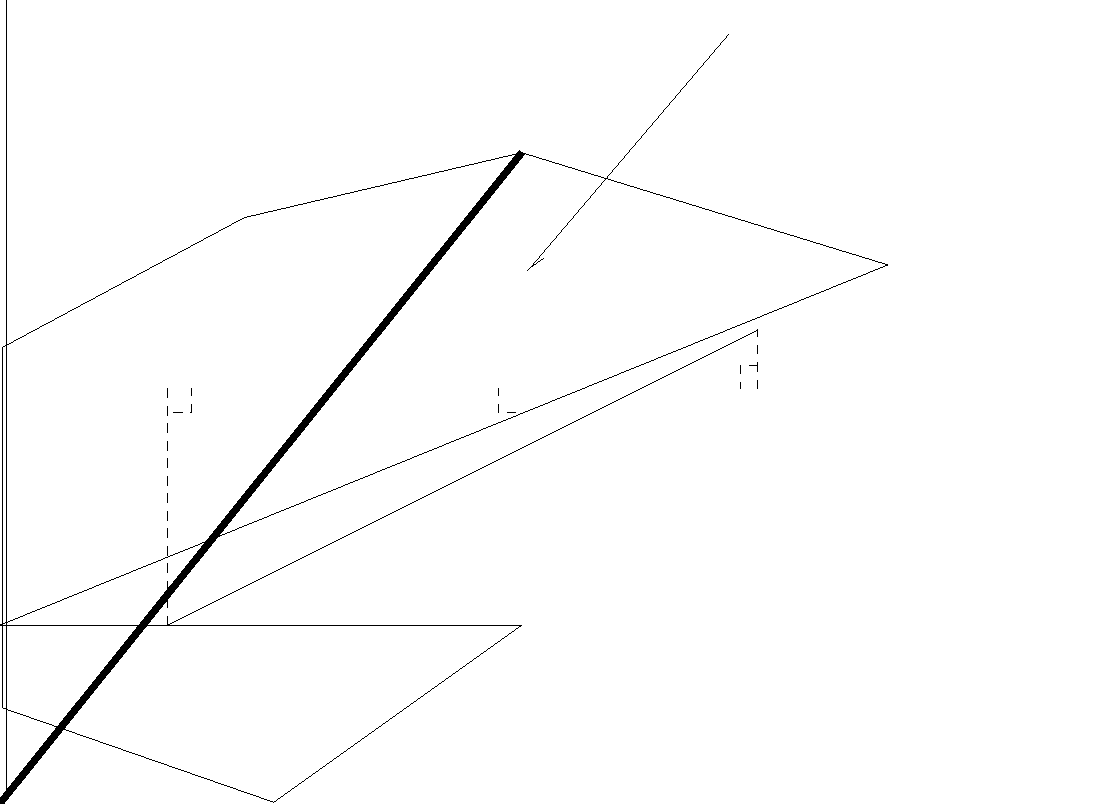
\includegraphics[height=4.5cm]{\repgraphics/facette}}}
\parbox{8cm}{\centerline{%
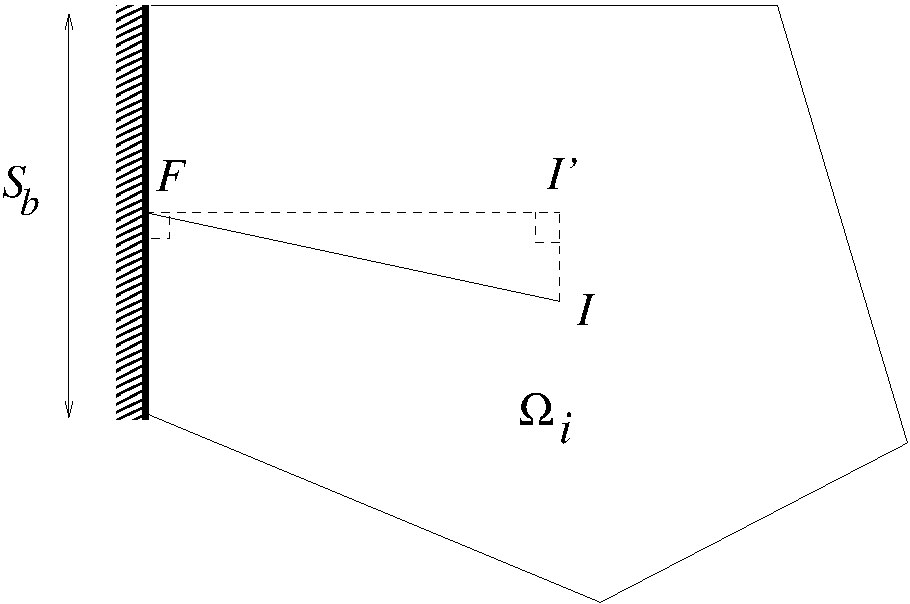
\includegraphics[height=4.5cm]{\repgraphics/facebord}}}
\caption{Identification of the geometric entities for internal (left) and
boundary faces (right).}
\label{Base_Introd_fig_geom}
\end{figure}

\clearpage %%%%%%%%%%%%%%%%%%%%%%%%%%%%%%%%%%%
%%%%%%%%%%%%%%%%%%%%%%%%%%%%%%%%%%

\section{Calling tree}

%%%%%%%%%%%%%%%%%%%%%%%%%%%%%%%%%%%
%%%%%%%%%%%%%%%%%%%%%%%%%%%%%%%%%%%
%
Each sub-section of this document is associated with an important
subroutine. The full list of the subroutines described here is the
following: \fort{bilsc2} \fort{clptur} \fort{clsyvt} \fort{codits} %
\fort{condli} \fort{covofi} \fort{gradmc} \fort{gradrc} \fort{inimas} %
\fort{itrmas} \fort{matrix} \fort{navsto} \fort{preduv} \fort{recvmc} %
\fort{resolp} \fort{turbke} \fort{turrij} \fort{viscfa} \fort{visort} %
\fort{vissec}.

The table~\ref{Base_Introd_simple_calling_tree} presents their sequence within a time
step. This calling tree is only partial. In particular, it does not account
for the number of calls to each subroutine. Also, for the sake of clarity,
no reference has been made to the subroutines dedicated to the gradient
calculation (\fort{gradmc}, \fort{gradrc}), which are called very often. For
the same reason, the calls to \fort{bilsc2} (advection fluxes) and %
\fort{matrix} (matrix calculation) which are made from within \fort{codits}
(treatment of an advection equation with source terms) have not been
reported.

The sub-sections where important information can be found are indicated
below:\newline
\newline
\nl \newline
\textbf{Calculation of gradients}\newline
\hspace*{1cm}\fort{gradrc}\newline
\hspace*{1cm}\fort{gradmc}\newline
\textbf{Least square method}\newline
\hspace*{1cm}\fort{recvmc}\newline
\hspace*{1cm}\fort{gradmc}\newline
\textbf{Convective schemes}\newline
\hspace*{1cm}\fort{bilsc2}\newline
\textbf{Wall-laws} (for velocity and temperature)\newline
\hspace*{1cm}\fort{clptur}\newline
\hspace*{1cm}\fort{condli}\newline
\textbf{System solve} (incremental method)\newline
\hspace*{1cm}\fort{codits}\newline
\textbf{Calculation of the values at the faces} (not exhaustive)\newline
\hspace*{1cm}\fort{viscfa}\newline
\hspace*{1cm}\fort{visort}\newline

Finally, for the reader wishing to become more familiar with the methods
implemented in \CS\, it is recommended to begin with the study of the
advection equation for a scalar (\fort{covofi}) which is solved iteratively
using an incremental method (\fort{codits}). It will then be useful to look
at \fort{navsto} which briefly presents the solution of the system made up
of the mass and momentum equations.

\begin{table}[htp]
\underline{\textbf{Calculation of the physical properties}}\newline
\underline{\textbf{Boundary Conditions}}\newline
\hspace*{1cm}\fort{condli} \newline
\hspace*{1,5cm}\fort{clptur} \hspace*{1cm} ``turbulent'' conditions at the
wall\newline
\hspace*{1,5cm}\fort{clsyvt} \hspace*{1cm} symmetry conditions for the
vectors and the tensors\newline
\underline{\textbf{Navier-Stokes solution}}\newline
\hspace*{1cm}\fort{navsto}\newline
\hspace*{1,5cm}\textbf{Velocity prediction}\newline
\hspace*{2,0cm}\fort{preduv} \newline
\hspace*{2,5cm}\fort{vissec} \hspace*{1cm} momentum source terms related to
the \newline
\hspace*{4,5cm} \hspace*{1cm} transposed gradient of the velocity\newline
\hspace*{2,5cm}\fort{viscfa} \hspace*{1cm} calculation of the viscosity at
the faces\newline
\hspace*{2,5cm}\fort{codits} \hspace*{1cm} iterative solution of the system
using an incremental method\newline
\hspace*{1,5cm}\textbf{Pressure correction}\newline
\hspace*{2,0cm}\fort{resolp} \newline
\hspace*{2,5cm}\fort{viscfa} \hspace*{1cm}calculation of the time step at
the faces...\newline
\hspace*{2,5cm}\fort{visort} \hspace*{1,5cm} ...according to the selected
options\newline
\hspace*{2,5cm}\fort{matrix} \hspace*{1cm}calculation of the Poisson
equation matrix\newline
\hspace*{2,5cm}\fort{inimas} \hspace*{1cm}initialisation of the mass flow
rate\newline
\hspace*{2,5cm}\fort{itrmas} \hspace*{1cm}update of the mass flow rate%
\newline
\hspace*{1,5cm} \textbf{Velocity correction}\newline
\hspace*{3,2cm} \hspace*{1cm}standard method or...\newline
\hspace*{2,0cm}\fort{recvmc} \hspace*{1cm}least square method\newline
\underline{\textbf{$k-\varepsilon$ model}}\newline
\hspace*{1cm}\fort{turbke}\newline
\hspace*{1,5cm}\fort{viscfa} \hspace*{1cm}preliminary steps before...\newline
\hspace*{1,5cm}\fort{bilsc2} \hspace*{1,5cm}...source terms coupling\newline
\hspace*{1,5cm}\fort{viscfa} \hspace*{1cm}calculation of the viscosity at
the faces\newline
\hspace*{1,5cm}\fort{codits} \hspace*{1cm}iterative solution of the systems
using an incremental method\newline
\underline{\textbf{Reynolds stress model}}\newline
\hspace*{1cm}\fort{turrij}\newline
\hspace*{1,5cm}\fort{visort} \hspace*{1cm}calculation of the viscosity at
the faces\newline
\hspace*{1,5cm}\fort{codits} \hspace*{1cm}iterative solution of the systems
using an incremental method\newline
\underline{\textbf{Equations for the scalars}}\newline
\hspace*{1cm}\fort{covofi}\newline
\hspace*{1,5cm}\fort{viscfa} \hspace*{1cm}calculation of the viscosity at
the faces\newline
\hspace*{1,5cm}\fort{codits} \hspace*{1cm}iterative solution of the systems
using an incremental method\newline
\caption{Partial and simplified calling tree associated with the successive
stages within a time step.}
\label{Base_Introd_simple_calling_tree}
\end{table}
